% Section content template for individual Educative lessons
% This file contains the actual content for a specific section
% Generated from Educative API section content

% Section: Requirements for the Online Blackjack Game
% Section ID: 6503083804983296
% Section Slug: requirements-for-the-online-blackjack-game
% Generated: 2025-12-12T12:54:31.390911

This lesson outlines the functional and operational requirements for the online Blackjack game. Identifying and understanding requirements is essential to defining the system's scope and ensuring a robust, user-friendly design.
\\
We'll use the notational convention to identify each requirement with a unique label ``Rn,'' where ``R'' is short for requirement and ``n'' is a natural number.

\subsection{Requirement collection}\label{CMgHu2Xd2kn27aWqIMEwk}
\\
The requirements for the Blackjack design problem are defined below:

\begin{itemize}
\item
\protect\phantomsection\label{fKwgomGvBPEdgQJUnj3kg}
\textbf{R1:} The system must support a shoe containing one or more standard decks of cards.
\item
\protect\phantomsection\label{rrJpbC7ZZTAJrC7opkR4D}
\textbf{R2:} Each deck consists of 52 cards in four suits (Hearts, Diamonds, Clubs, Spades), each containing 13 ranks: Ace, 2--10, Jack, Queen, and King.
\item
\protect\phantomsection\label{CGWu92LqtM_FG7AC4dUXC}
\textbf{R3:} Every card has a specific point value:
\end{itemize}

\begin{center}
{\def\LTcaptype{none} % do not increment counter
\begin{longtable}[]{@{}
>{\raggedright\arraybackslash} p{(\linewidth - 2\tabcolsep) * \real{0.5000}}
>{\raggedright\arraybackslash} p{(\linewidth - 2\tabcolsep) * \real{0.5000}}@{}}
\toprule\noalign{}
\endhead
\bottomrule\noalign{}
\endlastfoot
\begin{minipage}[t]{\linewidth}\raggedright
\textbf{Card}
\end{minipage} & \begin{minipage}[t]{\linewidth}\raggedright
\textbf{Face Value}
\end{minipage} \\
\begin{minipage}[t]{\linewidth}\raggedright
Ace
\end{minipage} & \begin{minipage}[t]{\linewidth}\raggedright
1 or 11
\end{minipage} \\
\begin{minipage}[t]{\linewidth}\raggedright
From 2 to 10
\end{minipage} & \begin{minipage}[t]{\linewidth}\raggedright
Equals the card number
\end{minipage} \\
\begin{minipage}[t]{\linewidth}\raggedright
Face cards (King, Queen, and Jack)
\end{minipage} & \begin{minipage}[t]{\linewidth}\raggedright
10
\end{minipage} \\
\end{longtable}
}
\end{center}

\begin{itemize}
\item
\textbf{R4:} The game has two user roles: the player and the dealer.
\item
\textbf{R5:} Each player must place a bet at the start of every round.
\item
\textbf{R6:} At the start of each game round, the dealer deals two cards to each player and two to themselves.
\item
\protect\phantomsection\label{oobzkSQNZf5JRVX0Xv33G}
\textbf{R7:} Both player cards are dealt face up; the dealer's first card is face up, and the second is face down.
\end{itemize}

\begin{figure}[htbp]
 \centering
 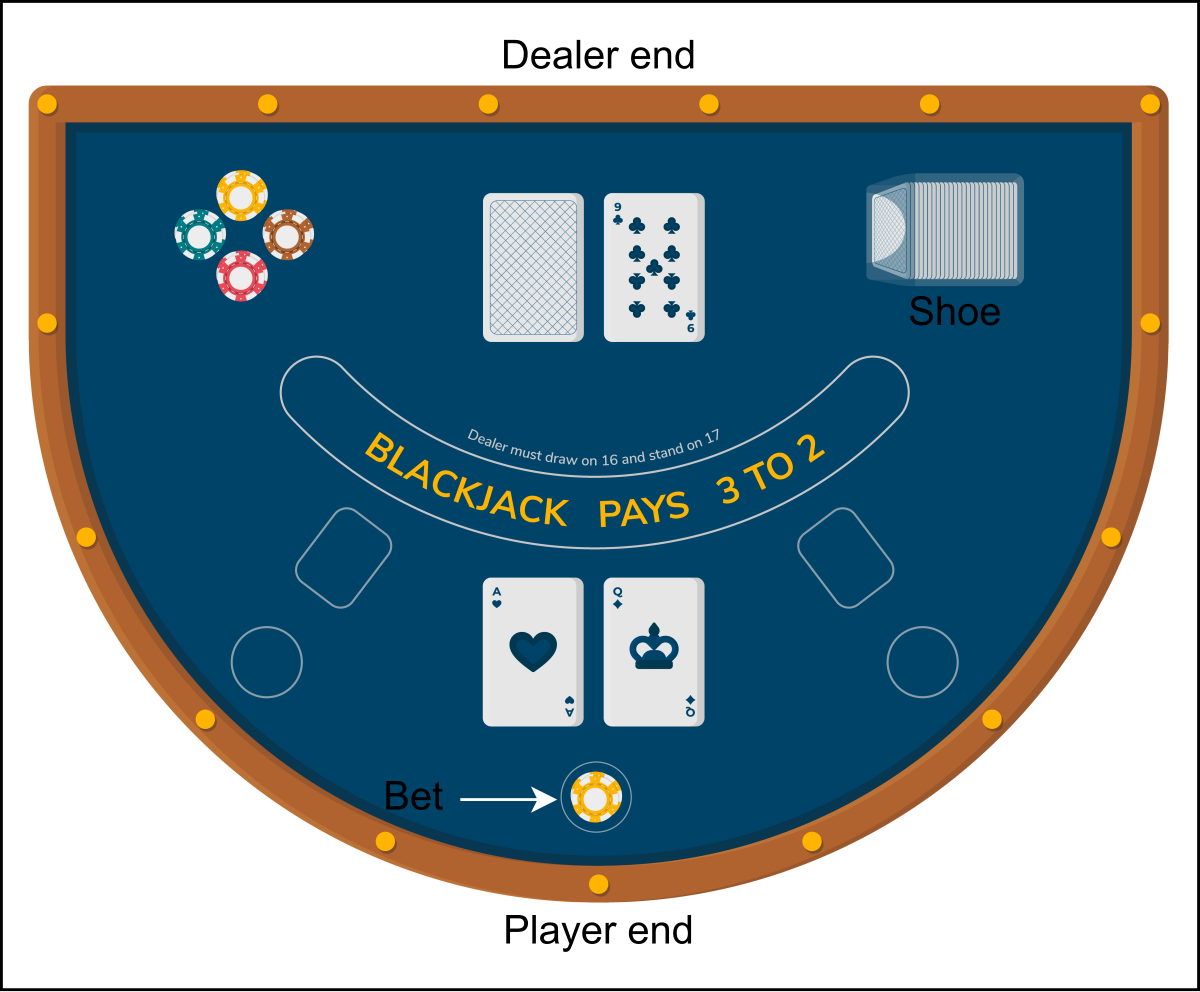
\includegraphics[width=0.5\textwidth]{Images/chapter_12/section_6503083804983296/5118448909942784.png}
 
\end{figure}

\begin{itemize}
\item
\protect\phantomsection\label{S51ibNGMVDsZf4qy6aC9S}
\textbf{R8:} Players may hit (draw an additional card) if their hand total is less than 21 points.
\item
\protect\phantomsection\label{NSAf8HCxC3XN7SfkKl0o3}
\textbf{R9:} According to standard Blackjack rules, the dealer must hit if their hand value exceeds 17 points.
\item
\protect\phantomsection\label{SrW_9q4WKq-eTJY1EuHA5}
\textbf{R10:} If a player's or dealer's hand exceeds 21 points, they bust and immediately lose that round.
\item
\protect\phantomsection\label{QjVb8iEQE1lL4j7P2LkR4}
\textbf{R11:} Players may stand (decline to take more cards) at any time during their turn.
\item
\protect\phantomsection\label{ixuoyi0RD-0H-Hpwhq9Tz}
\textbf{R12:} At the end of the round, if a player's hand total is higher than the dealer's and does not exceed 21, the player wins and receives a payout equal to their bet (1:1).
\item
\protect\phantomsection\label{px9sUqxDBo1LmKbP0H9jc}
\textbf{R13:} If a player achieves a Blackjack (Ace and a 10-point card as their initial two cards), they receive a payout of 3:2 (150\% of their bet).
\item
\protect\phantomsection\label{FftfEc6hP9ExdKS6TRj3m}
\textbf{R14:} If the player and dealer have the same point total at the end of a round, it is a push; the player gets their original bet back, or may be offered a replay.
\item
\protect\phantomsection\label{vBcHXepyXz5YezTS0hsRF}
\textbf{R15:} If a player leaves or disconnects before the end of a round, the dealer automatically wins that round.
\end{itemize}
\\
We've identified our requirements for the problem, and in the next lesson, we will define different use cases for the online Blackjack game design.

% End of section content